\subsection{Embeddings}
Sparse to dense representation
One hot encoding vs embeddings
Word2Vec

\subsection{Activation function}
In a neural network activation functions are mathematical equations applied to each neuron and it determines if it should activate or not based on its inputs. This function must be computationally efficient to calculate and will generally be non-linear. The last part is very important because without non-linearities a NN would just behave like a single-layer perceptron and would not we able to model complex functions. One exception to this is the output layer for a regression NN which will have a linear activation in order to allow the prediction of any real value as.

Early neural networks were using tanh and sigmoid activation functions. Sigmoid also known as logistic function is S shaped and bounded above by 1 and below by 0 
% Simply put an activation function decides if a neuron should `fire`
Traditional sigmoid \ref{eq:sigmoid}, tanh \ref{eq:tanh}

Rectified Linear Unit ReLU \ref{eq:relu}
A major drawback of using ReLU activations is the "dying ReLU" problem.  
leaky ReLU \ref{eq:leakyrelu}
comparison with traditional ones
comparison between relu and leaky relu

\begin{equation}
    \label{eq:sigmoid}
    \begin{aligned}
    f(x) &= \frac{1}{1+e^{-x}} \\
    f'(x) &= f(x)(1 - f(x))
    \end{aligned}
\end{equation}

\begin{equation}
    \label{eq:tanh}
    \begin{aligned}
    f(x) &= \frac{2}{1+e^{-2x}} - 1 \\
    f'(x) &= 1 - f(x)^2
    \end{aligned}
\end{equation}

\begin{equation}
    \label{eq:relu}
    \begin{aligned}
    f(x) &=
    \begin{cases}
        x, & \text{if } x\geq 0 \\
        0, & \text{otherwise}
    \end{cases} \\
    f'(x) &=
    \begin{cases}
        1, & \text{if } x\geq 1 \\
        0, & \text{otherwise}
    \end{cases}
    \end{aligned}
\end{equation}

\begin{equation}
    \label{eq:leakyrelu}
    \begin{aligned}
    f(x) &=
    \begin{cases}
        x, & \text{if } x\geq 0 \\
        0.01x, & \text{otherwise}
    \end{cases} \\
    f'(x) &=
    \begin{cases}
        1, & \text{if } x\geq 1 \\
        0.01, & \text{otherwise}
    \end{cases}
    \end{aligned}
\end{equation}

% \begin{figure}[h!]
%     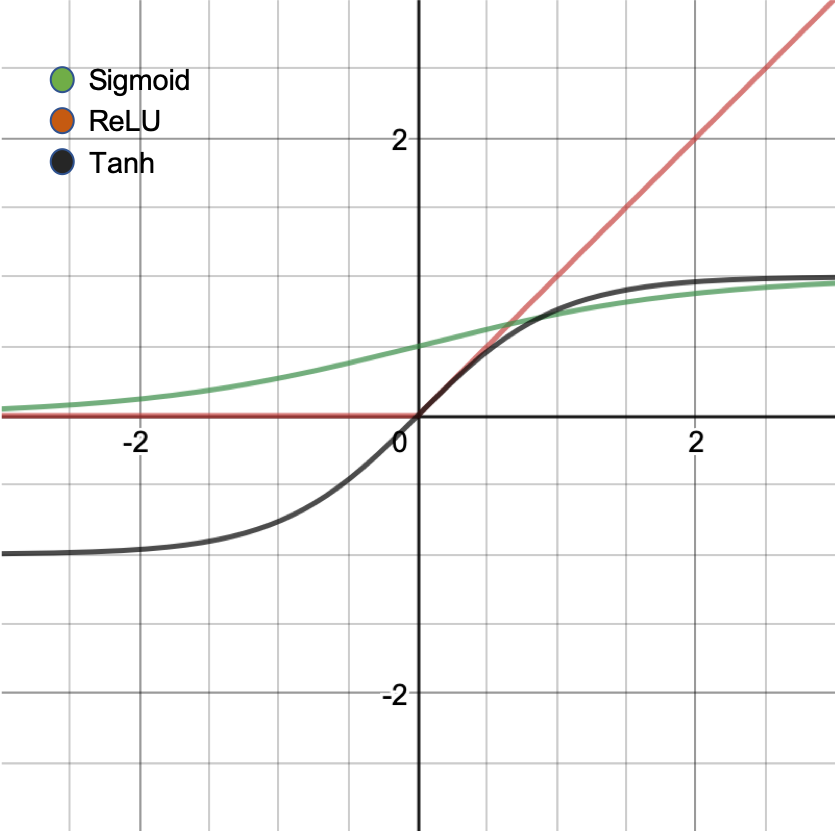
\includegraphics[scale=0.5]{3-activation-func.png}
%     \caption{Activation functions comparison}
% \end{figure}

% \begin{figure}[h!]
%     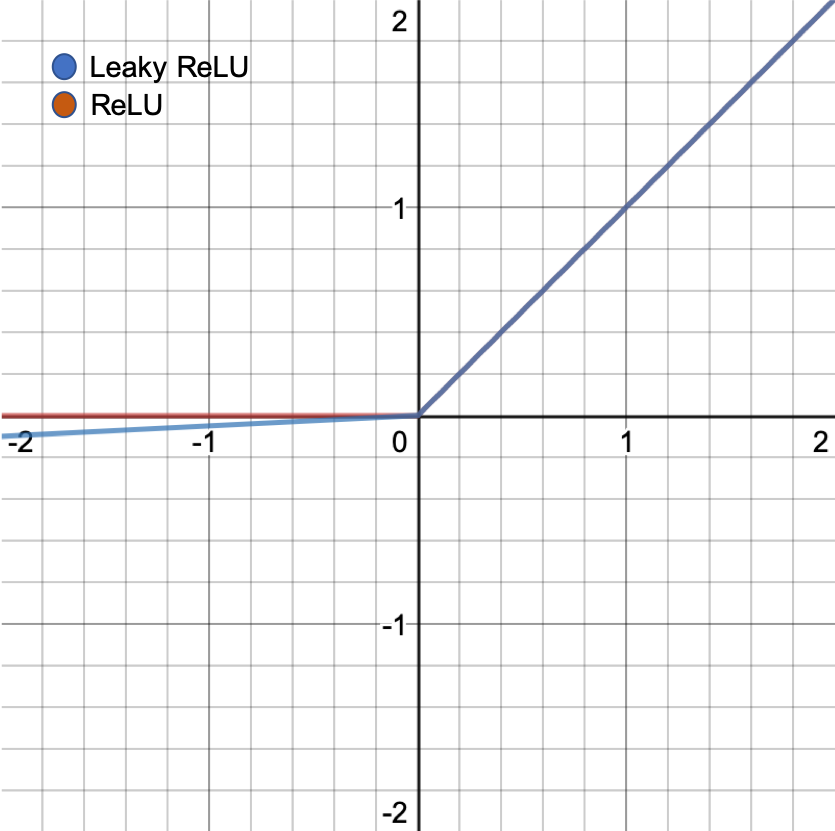
\includegraphics[scale=0.5]{leakyReLUvsReLU.png}
%     \caption{Leaky ReLU vs ReLU}
% \end{figure}

\begin{figure}[h!]
    \subfloat[Activation functions]{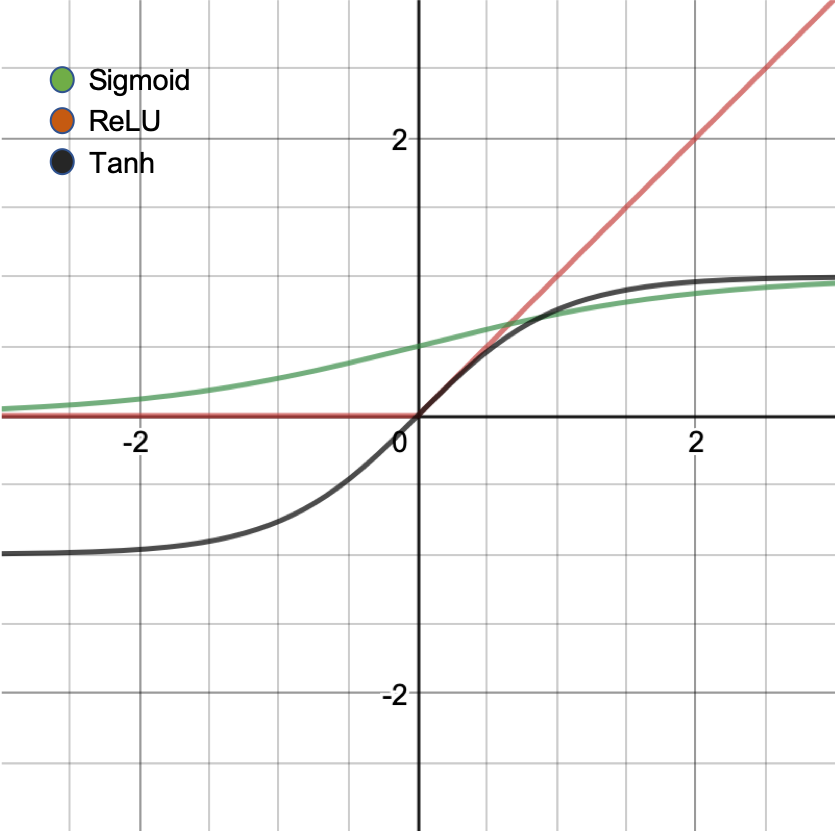
\includegraphics[scale=0.5]{3-activation-func}\label{fig:activations}}
    \hfill
    \subfloat[ReLU vs Leaky ReLU]{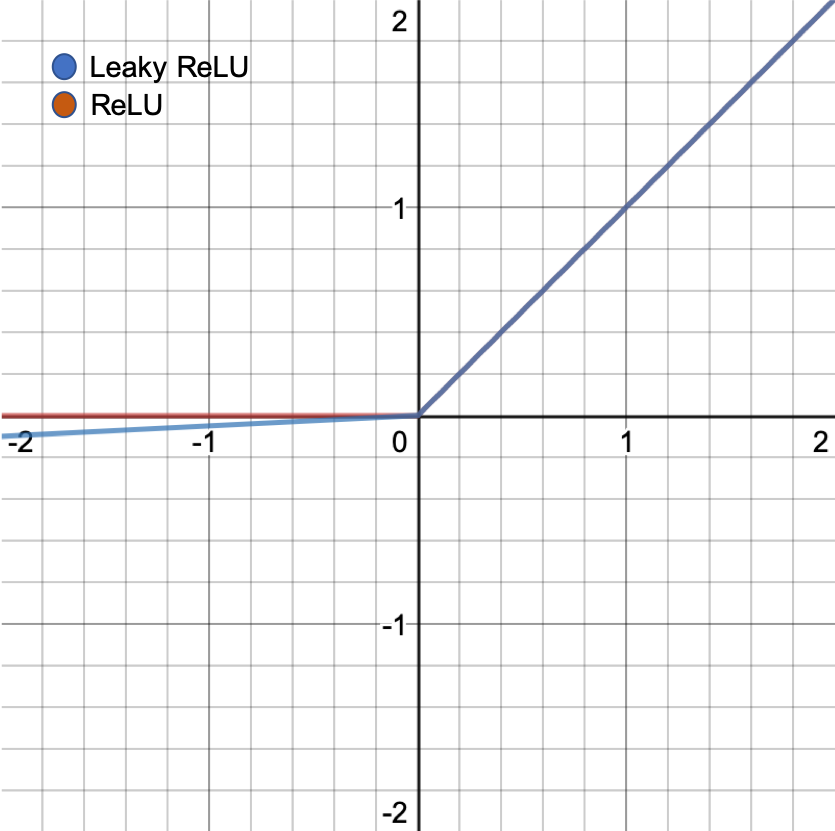
\includegraphics[scale=0.5]{leakyReLUvsReLU}\label{fig:relus}}
\end{figure}


\subsection{Regularization}
Kernel Regularization
Activity Regularization
Dropout general value 0.5 gives higher RMSE than 0.2
% A dropout rate of 0.2 was found to be better and result in a \% decrease in RMSE than the generally used 0.5. 

\subsection{Optimizer}
Optimizers are a very important parameter in NN configuration. Nowadays theres a vast choice of good optimizers. At its core an optimizer is an iterative method of optimizing for a cost function. At each step of the optimization the weights in the NN will be updated based on the negative of the gradient of the cost function. Stochastic gradient descent (SGD) is a variation of GD in that the optimization happens after each training example. In practice this usually implies mini-batches of between 32 and 1024 data points. Batch gradient descent involves updating the weights based on the gradient over the whole dataset. SGD optimizes based on an approximation of the gradient unlike batch gradient descent. This turns out to be useful as it introduces noise in the network which leads to better generalization. It is also more scalable as the whole dataset does not have to be kept in memory.

% It is well studied and its convergence is mathematically provable. 
\begin{equation}
    \theta = \theta - \alpha \Delta_{\theta} J(\theta ;x^{(i)}y^{(i)})
\end{equation}

More advanced optimizers are built on top of SGD and include things such as adaptive learning rates and momentum to increase convergence speed and overall stability.

One such algorithm is adaptive moment estimation (Adam). Its widely used in literature and much faster than SGD

Nesterov accelerated gradient
Adaptive Moment Estimation (Adam) 
Adam can be seen as a combination of RMSProp and momentum. \citet{Adam}
Nesterov adaptive moment estimation (NAdam) combines adam with nesterov momentum which improve convergence (cite)

\subsection{Serving recommendation \& Api}
Structure of Api.
Create pod that just retrains the model on new ratings. Once finished redeploy pods